% Options for packages loaded elsewhere
\PassOptionsToPackage{unicode}{hyperref}
\PassOptionsToPackage{hyphens}{url}
%
\documentclass[
  a4paper,
]{article}
\usepackage{amsmath,amssymb}
\usepackage{setspace}
\usepackage{iftex}
\ifPDFTeX
  \usepackage[T1]{fontenc}
  \usepackage[utf8]{inputenc}
  \usepackage{textcomp} % provide euro and other symbols
\else % if luatex or xetex
  \usepackage{unicode-math} % this also loads fontspec
  \defaultfontfeatures{Scale=MatchLowercase}
  \defaultfontfeatures[\rmfamily]{Ligatures=TeX,Scale=1}
\fi
\usepackage{lmodern}
\ifPDFTeX\else
  % xetex/luatex font selection
\fi
% Use upquote if available, for straight quotes in verbatim environments
\IfFileExists{upquote.sty}{\usepackage{upquote}}{}
\IfFileExists{microtype.sty}{% use microtype if available
  \usepackage[]{microtype}
  \UseMicrotypeSet[protrusion]{basicmath} % disable protrusion for tt fonts
}{}
\makeatletter
\@ifundefined{KOMAClassName}{% if non-KOMA class
  \IfFileExists{parskip.sty}{%
    \usepackage{parskip}
  }{% else
    \setlength{\parindent}{0pt}
    \setlength{\parskip}{6pt plus 2pt minus 1pt}}
}{% if KOMA class
  \KOMAoptions{parskip=half}}
\makeatother
\usepackage{xcolor}
\usepackage[margin=1in]{geometry}
\usepackage{longtable,booktabs,array}
\usepackage{calc} % for calculating minipage widths
% Correct order of tables after \paragraph or \subparagraph
\usepackage{etoolbox}
\makeatletter
\patchcmd\longtable{\par}{\if@noskipsec\mbox{}\fi\par}{}{}
\makeatother
% Allow footnotes in longtable head/foot
\IfFileExists{footnotehyper.sty}{\usepackage{footnotehyper}}{\usepackage{footnote}}
\makesavenoteenv{longtable}
\usepackage{graphicx}
\makeatletter
\def\maxwidth{\ifdim\Gin@nat@width>\linewidth\linewidth\else\Gin@nat@width\fi}
\def\maxheight{\ifdim\Gin@nat@height>\textheight\textheight\else\Gin@nat@height\fi}
\makeatother
% Scale images if necessary, so that they will not overflow the page
% margins by default, and it is still possible to overwrite the defaults
% using explicit options in \includegraphics[width, height, ...]{}
\setkeys{Gin}{width=\maxwidth,height=\maxheight,keepaspectratio}
% Set default figure placement to htbp
\makeatletter
\def\fps@figure{htbp}
\makeatother
\setlength{\emergencystretch}{3em} % prevent overfull lines
\providecommand{\tightlist}{%
  \setlength{\itemsep}{0pt}\setlength{\parskip}{0pt}}
\setcounter{secnumdepth}{-\maxdimen} % remove section numbering
\ifLuaTeX
\usepackage[bidi=basic]{babel}
\else
\usepackage[bidi=default]{babel}
\fi
\babelprovide[main,import]{catalan}
% get rid of language-specific shorthands (see #6817):
\let\LanguageShortHands\languageshorthands
\def\languageshorthands#1{}
\ifLuaTeX
  \usepackage{selnolig}  % disable illegal ligatures
\fi
\usepackage{bookmark}
\IfFileExists{xurl.sty}{\usepackage{xurl}}{} % add URL line breaks if available
\urlstyle{same}
\hypersetup{
  pdftitle={U3. WINDOWS SERVER. ADMINISTRACIÓ I CONFIGURACIÓ (IV)},
  pdfauthor={@tofermos 2024},
  pdflang={ca-ES},
  hidelinks,
  pdfcreator={LaTeX via pandoc}}

\title{U3. WINDOWS SERVER. ADMINISTRACIÓ I CONFIGURACIÓ (IV)}
\usepackage{etoolbox}
\makeatletter
\providecommand{\subtitle}[1]{% add subtitle to \maketitle
  \apptocmd{\@title}{\par {\large #1 \par}}{}{}
}
\makeatother
\subtitle{SERVEI DHCP}
\author{@tofermos 2024}
\date{}

\begin{document}
\maketitle

{
\setcounter{tocdepth}{2}
\tableofcontents
}
\setstretch{1.5}
\newpage
\renewcommand\tablename{Tabla}

\section{1 Servei de DHCP}\label{servei-de-dhcp}

Es tracta de la funció bàsica de proporcionar IP provades en les LAN .
Encara que aquest servei en altres tipus de xarxes el donen diferents
dispositius com és el cas de les WIFIS públiques o el router domèstic.

\subsection{1.1 Conceptes previs}\label{conceptes-previs}

\begin{verbatim}
Recordatori:  Conceptes del mòdul de XAL de 1r SMX

- Adreça IP: Una adreça única dins del rang establit pel servidor.

- Màscara de subxarxa: Indica la porció de la xarxa a la qual pertany l'adreça IP.

- Adreça MAC: Adreça única de cada dispositiu (tarja ethernet, WIFI o boca d'un switch). Conté 6 bytes, els 3 més alts identifiquen el fabricant. Els altres 3, al dipositiu de forma única.

- Passarel·la predeterminada: Normalment, és l'adreça del router o un altre dispositiu de xarxa que connecta la xarxa local amb Internet.

-Servidors DNS: Les adreces dels servidors que resolen els noms de domini a adreces IP.
\end{verbatim}

El servei \textbf{DHCP (Dynamic Host Configuration Protocol)} en
\textbf{Windows Server} és una \textbf{funció de servidor} que permet
als administradors de xarxa automatitzar l'assignació d'adreces IP i
altres paràmetres de configuració de xarxa als dispositius que es
connecten a la xarxa.

\subsection{1.2 Funcionament del servei
DHCP}\label{funcionament-del-servei-dhcp}

Aquesta funció s'implementa en Windows Server com un servici que respon
a la filosofia del model client servidor. Quan un dispositiu (com un
ordinador, càmera IP, mòbil, impressora\ldots) es connecta a la xarxa,
envia una sol·licitud per obtenir una adreça IP. El servidor DHCP respon
a aquesta petició assignant-li una adreça IP de manera automàtica i
dinàmica, així com altres paràmetres de configuració de xarxa com:

\begin{enumerate}
\def\labelenumi{\arabic{enumi}.}
\tightlist
\item
  \textbf{Discover}: El client envia una petició en difusió per trobar
  un servidor DHCP a la xarxa.
\item
  \textbf{Offer}: El servidor DHCP respon oferint una adreça IP.
\item
  \textbf{Request}: El client accepta l'oferta enviant una sol·licitud
  per a l'adreça IP.
\item
  \textbf{Acknowledge}: El servidor DHCP confirma l'assignació de
  l'adreça IP al client.
\end{enumerate}

\begin{figure}
\centering
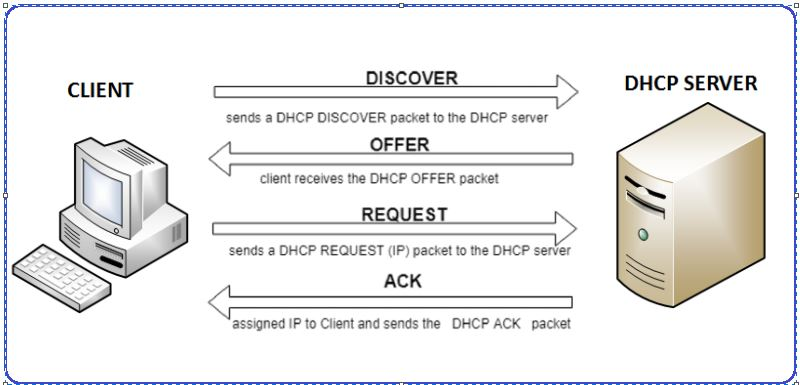
\includegraphics[width=0.6\textwidth,height=\textheight]{png/DHCPesquema.jpg}
\caption{\emph{Figura1: Esquema C/S}}
\end{figure}

\subsection{1.3 Elements principals del
DHCP}\label{elements-principals-del-dhcp}

\begin{itemize}
\item
  \textbf{Rangs o àmbits}: Conjunt o rang d'adreces IP que es poden
  assignar als dispositius clients.
\item
  \textbf{Exclusions}: Quan volem que dins del rang alguna IP o grup
  d'IPs (``subrangs'') no s'assignen. Pot ser útil per si volem
  assignar-les de forma manual a determinats dipositius.
\item
  \textbf{Reserves}: IP que el DHCP assigna sempre al matei dispositiu.
  Es basa en la seua MAC.
\item
  \textbf{Opcions DHCP}: Paràmetres addicionals, com ara passarel·les
  (router o gateway) predeterminades o DNS, que el servidor DHCP pot
  proporcionar als dispositius clients.
\end{itemize}

En resum, el servei DHCP en Windows Server facilita la gestió i
assignació automàtica d'adreces IP en una xarxa, millorant l'eficiència
i reduint la complexitat de la configuració manual de xarxes.

\section{2 Implementació en Windows Server
2019}\label{implementaciuxf3-en-windows-server-2019}

Veiem com s'implementa aquesta funció típica d'un model Client/Servidor
el Windwos Server 2019.

\subsection{2.1 Instal·lació}\label{installaciuxf3}

Un dels servicis més típics i usats d'un servidor senzill de xarxa és
l'assignació dinàmica de IP privades de la xarxa local. Veiem com
instal·lem i configurem el servei.

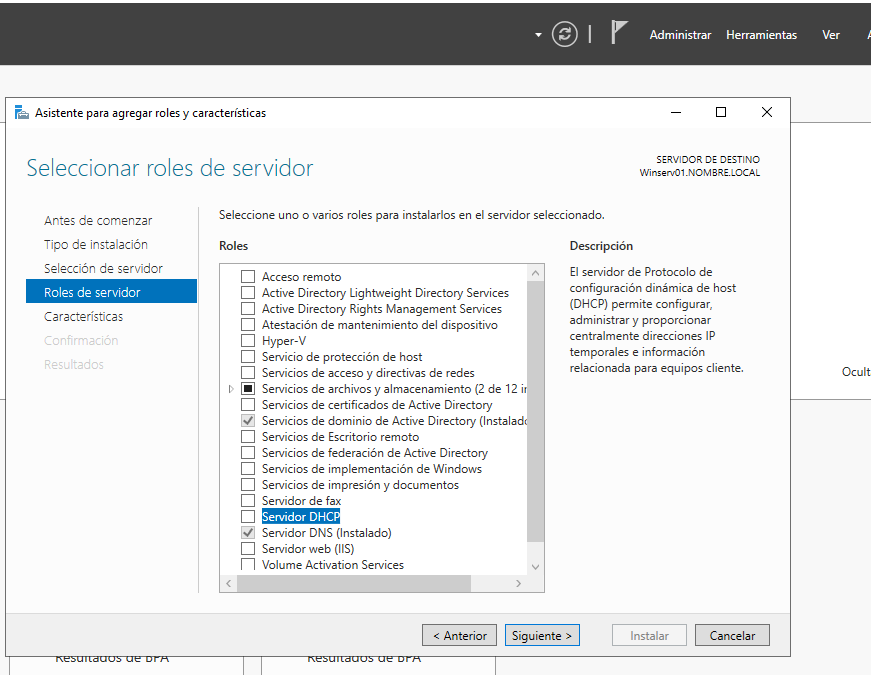
\includegraphics[width=0.6\textwidth,height=\textheight]{png/DHCP1.png}

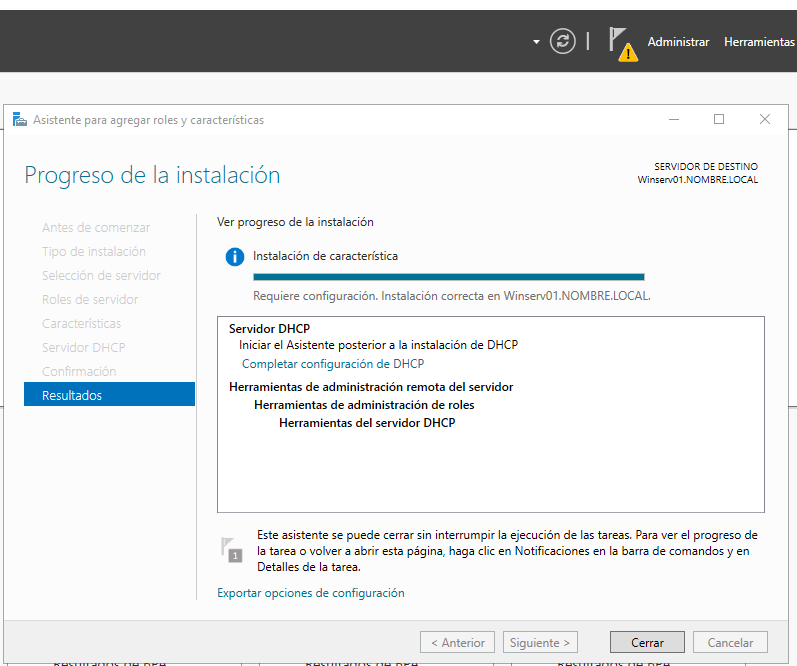
\includegraphics[width=0.6\textwidth,height=\textheight]{png/DHCP2.png}

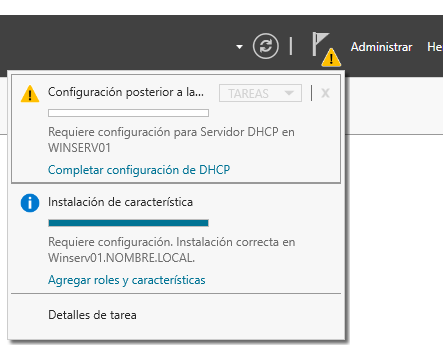
\includegraphics[width=0.6\textwidth,height=\textheight]{png/DHCP3.png}

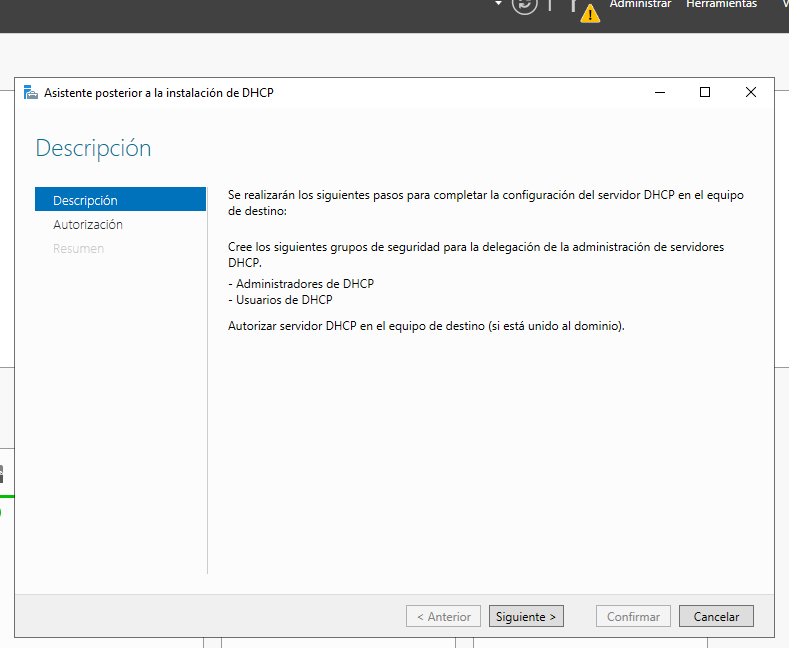
\includegraphics[width=0.6\textwidth,height=\textheight]{png/DHCP4.png}

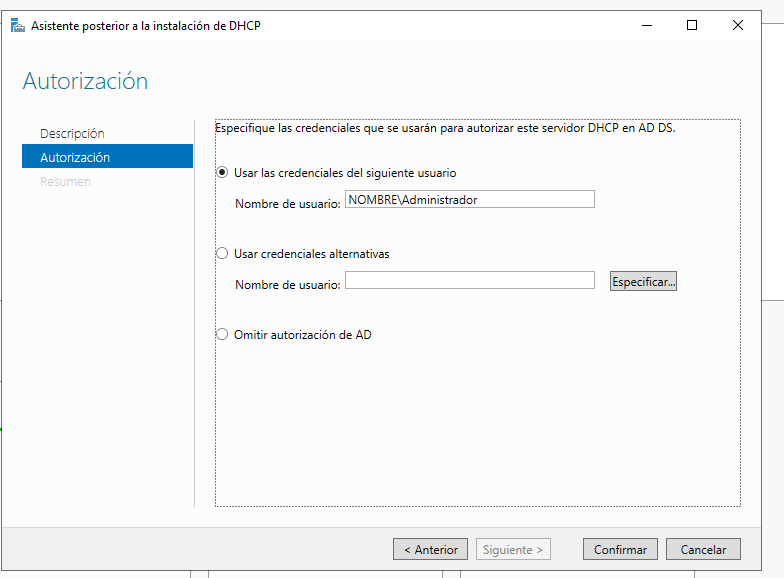
\includegraphics[width=0.6\textwidth,height=\textheight]{png/DHCP5.png}

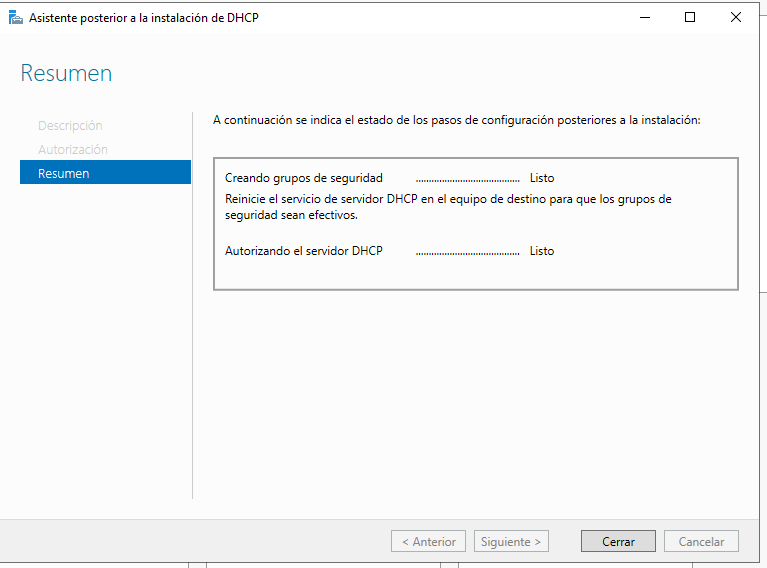
\includegraphics[width=0.6\textwidth,height=\textheight]{png/DHCP6.png}

\subsection{2.2 Configuració}\label{configuraciuxf3}

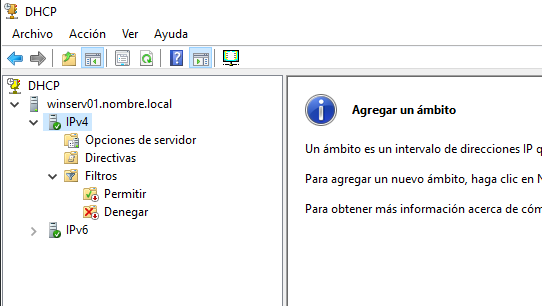
\includegraphics[width=0.6\textwidth,height=\textheight]{png/DHCP7.png}

\subsubsection{Creem un rang de IP}\label{creem-un-rang-de-ip}

\textbf{Pasos recomanables} * El/s rang/s ha d'abarcar TOTES les volem a
la xarxa local. Després indicarem (dins de rang) quines queden excloses:
* Exclourem les que vulguem assignar manualment (estàtiques)\ldots{} (
servidors, altres routers\ldots). Vorem que el servidor DNS i el Gateway
(encaminador) ens el demana ara. * Exclourem les que posem a disposició
d'altri (administrador extern de fotocopiadores de xarxa o de càmeres
IP, per exemple). * Fer les reserves de IP per a determinades MAC:
Assignem les IP ( dinàmica) però constant a un dispositiu en concret

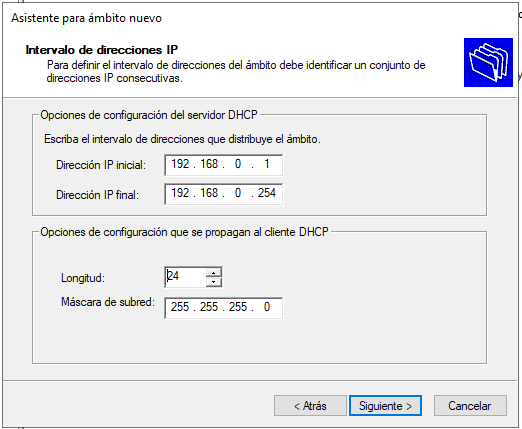
\includegraphics[width=0.6\textwidth,height=\textheight]{png/DHCP8.png}

\subsubsection{Exclusions}\label{exclusions}

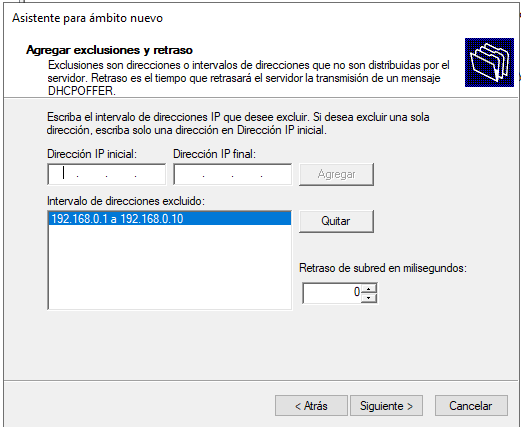
\includegraphics[width=0.6\textwidth,height=\textheight]{png/DHCP9.png}

\subsubsection{Duració de
l'assignació}\label{duraciuxf3-de-lassignaciuxf3}

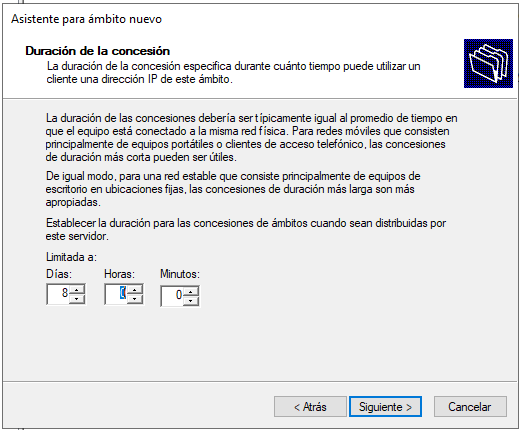
\includegraphics[width=0.6\textwidth,height=\textheight]{png/DHCP10.png}

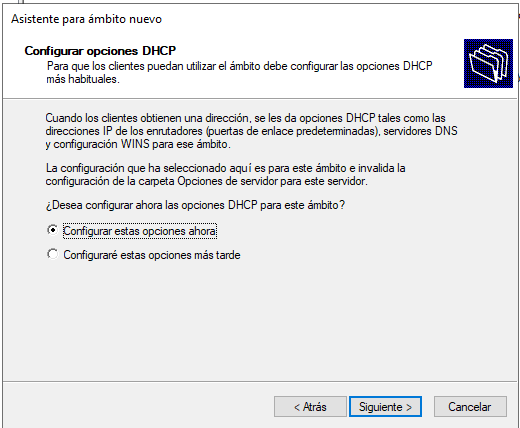
\includegraphics[width=0.6\textwidth,height=\textheight]{png/DHCP11.png}

\subsubsection{Gateway (porta d'enllaç) o
encaminador}\label{gateway-porta-denllauxe7-o-encaminador}

Indiquem la IP que hem configurat al router.

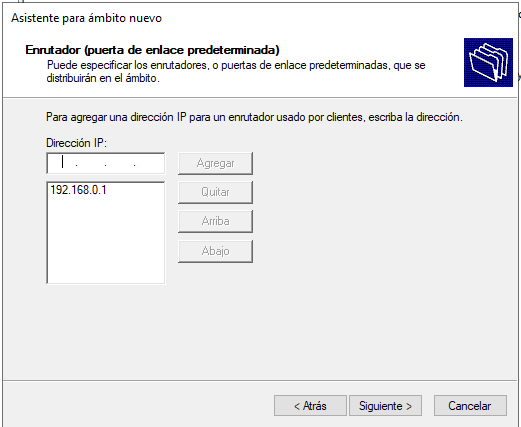
\includegraphics[width=0.6\textwidth,height=\textheight]{png/DHCP12.png}

\subsubsection{Servidor DNS}\label{servidor-dns}

Indiquem la IP que té el servidor amb el servei DNS.

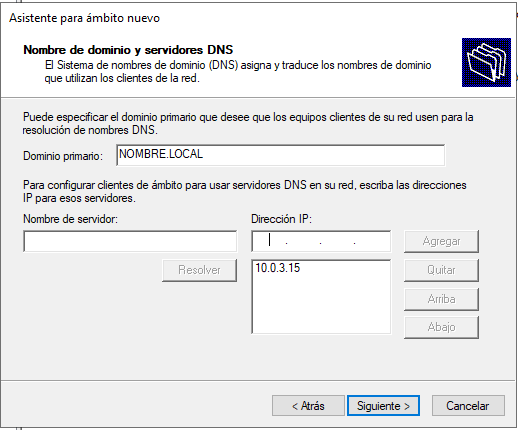
\includegraphics[width=0.6\textwidth,height=\textheight]{png/DHCP13.png}

\section{3 DHCP com servei}\label{dhcp-com-servei}

Mirarem més avant els servicis però podem observar ja alguna
característica típica d'este software de servidor. Entrem a la consola
de Serveis (\textbf{services.msc}):

\begin{itemize}
\tightlist
\item
  Podem reiniciar-lo o aturar-lo
\end{itemize}

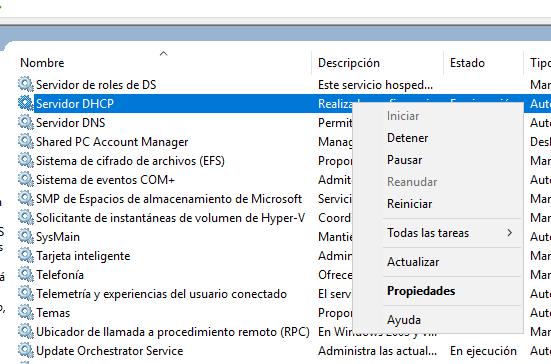
\includegraphics[width=0.6\textwidth,height=\textheight]{png/ServiciDHCP0.png}

\begin{itemize}
\tightlist
\item
  El tipus d'inici per defecte és, obviament, automàtic
\end{itemize}

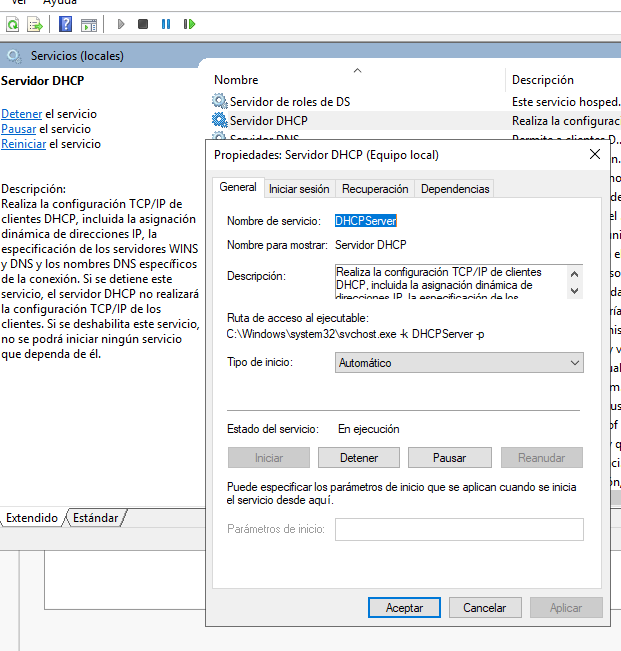
\includegraphics[width=0.6\textwidth,height=\textheight]{png/ServiciDHCP1.png}

\begin{itemize}
\item
  No està associat a cap compte d'usuari en concret que haja d'iniciar
  sessió

  Només cal iniciar sessió en un servidor puntualment per a tasques de
  manteniment.
\end{itemize}

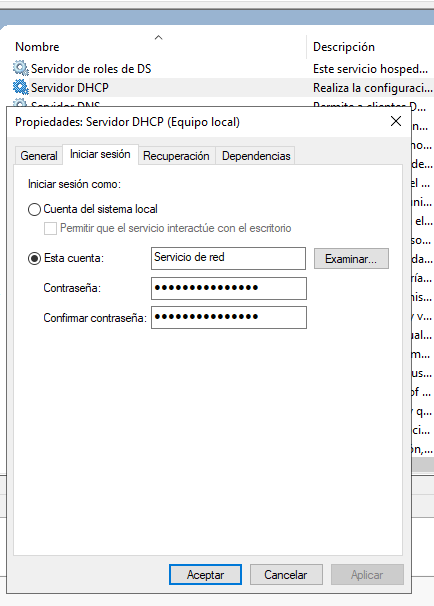
\includegraphics[width=0.6\textwidth,height=\textheight]{png/ServiciDHCP2.png}

\section{4 Client}\label{client}

En el client devem canviar la configuració de la NIC i especificar que,
ara, la IP l'assignarà el DHCP

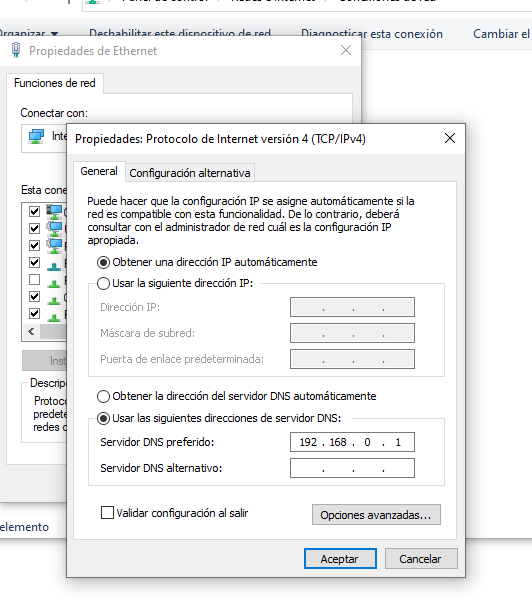
\includegraphics[width=0.6\textwidth,height=\textheight]{png/DHCP14.png}

\subsection{4.1 El servici DHCP en el
client.}\label{el-servici-dhcp-en-el-client.}

\begin{itemize}
\tightlist
\item
  L'assignació dinàmica de IP o protocol DHCP respon al \textbf{model
  client servidor}.
\item
  Altra qüestió és que la implementació del ``client DHCP'' en els PC
  satèlits o clients siga mitjançant un ``servei local de Windows''.
\item
  Per vore el software client, entrem en la consola de serveis:
  \textbf{services.msc}
\end{itemize}

\begin{longtable}[]{@{}
  >{\raggedright\arraybackslash}p{(\columnwidth - 4\tabcolsep) * \real{0.3333}}
  >{\raggedright\arraybackslash}p{(\columnwidth - 4\tabcolsep) * \real{0.3333}}
  >{\raggedright\arraybackslash}p{(\columnwidth - 4\tabcolsep) * \real{0.3333}}@{}}
\toprule\noalign{}
\begin{minipage}[b]{\linewidth}\raggedright
Model C/S
\end{minipage} & \begin{minipage}[b]{\linewidth}\raggedright
Nom del servici Windows
\end{minipage} & \begin{minipage}[b]{\linewidth}\raggedright
Acció
\end{minipage} \\
\midrule\noalign{}
\endhead
\bottomrule\noalign{}
\endlastfoot
Servidor DHCP & ``Servicio DHCP'' en Windows Server & Reb peticions de
IP de dispositius i les assigna \\
Client DHCP & ``Cliente DHCP'' en Windows 1x & Sol·licita IP i, en
rebre-la, la configura a la tarja \\
\end{longtable}

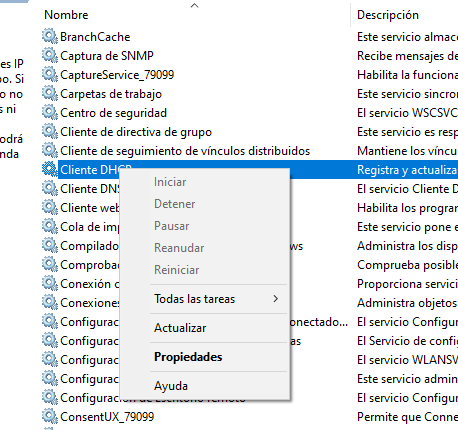
\includegraphics[width=0.6\textwidth,height=\textheight]{png/ServiciClientDHCP0.png}
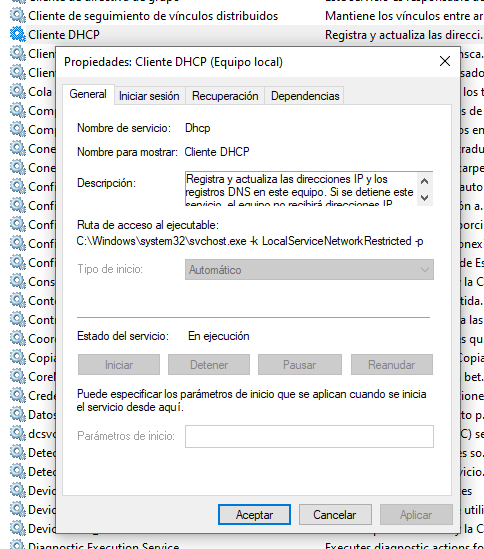
\includegraphics[width=0.6\textwidth,height=\textheight]{png/ServiciClientDHCP1.png}
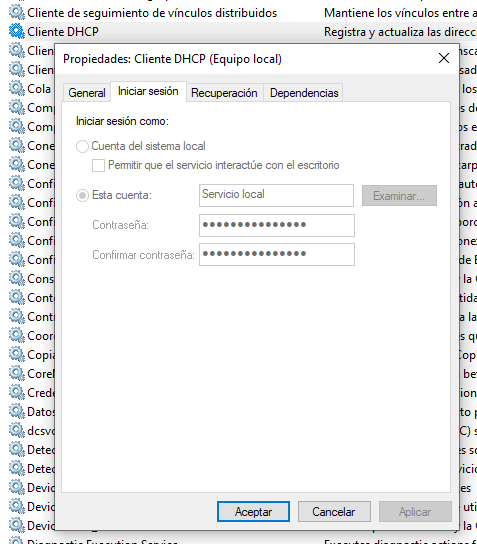
\includegraphics[width=0.6\textwidth,height=\textheight]{png/ServiciClientDHCP2.png}

\section{5 Avantatges del servei DHCP en Windows
Server}\label{avantatges-del-servei-dhcp-en-windows-server}

\begin{itemize}
\tightlist
\item
  \textbf{Gestió centralitzada}: DHCP facilita la gestió de les adreces
  IP des d'un servidor central, evitant la configuració manual de cada
  dispositiu.
\item
  \textbf{Eficàcia}: Assegura que no es produeixin conflictes d'adreces
  IP duplicades a la xarxa.
\item
  \textbf{Escalabilitat}: És especialment útil en xarxes grans, on
  assignar IPs manualment seria lent i poc pràctic.
\item
  \textbf{Flexibilitat}: Si volem un canvi de totes les IP o gran part,
  només hem de configurar-lo al servici i reiniciar el dispositius.
  Imaginem, per exmeple, passar de IPv4 de classe C a B per a tota una
  xarxa.
\item
  \textbf{Actualitzacions automàtiques}: El servidor DHCP pot canviar
  les adreces IP dels dispositius a mesura que es connecten i
  desconnecten de la xarxa.
\item
  \textbf{Concessió temporal d'adreces IP}: Les IPs es poden assignar
  amb una duració específica, de manera que quan un dispositiu deixa de
  ser necessari a la xarxa, l'IP es pot reutilitzar.
\end{itemize}

\end{document}
